\section{Sparqled: Query Recommendation}
\label{sec:exploiting:sparqled:recommendation}

When a user formulates a SPARQL query, the user is in fact trying to summarise his information needs. However, this task can be very difficult and time consuming as it requires the user to have a good knowledge of the structure and vocabulary of the dataset he is trying to query. This task becomes even more complex if the user is trying to formulate a query across multiple data sources. In order to gain such knowledge, the user must explore and investigate the data itself before querying it. To save the user from such a tedious work we develop an \emph{Assisted SPARQL Editor}, an application that leverages the data graph summary to help the user into effectively formulating complex SPARQL queries even without prior knowledge about the structure and vocabulary of the data sources. In this section, we first give an overview of the possible recommendations supported by the SPARQL editor. Then we introduce some of the main concepts in SPARQL before explaining how the current state of the SPARQL query is used to query the data graph summary and to retrieve possible structural query elements for recommendation.

\subsection{Recommendations Overview}

The Assisted SPARQL Editor supports four kinds of recommendations: class, predicate, relationships between variables and named graphs. Examples of such recommendations are pictured in Figure~\ref{fig:rkb-recommendations}. Recommendations of entity node labels as well as literal node labels are not supported since such content data is discarded from the data graph summary.

During query formulation, the assisted editor provides one of these four different types of recommendations to the user based on the state of the edited query. The state of the edited query is composed of an incomplete graph pattern and the cursor position. The cursor position materialises the \emph{Point Of Focus} (POF), i.e., the unknown element of the graph pattern for which the user requests recommendations. 

Figure~\ref{fig:rkb-recommendations-types} depicts the recommendations of possible classes for a variable. Given that the variable \emph{?Article} is associated to a predicate \emph{akt:hasAuthor}, the system will only recommend classes that are mentioned with this predicate in the data graph. Figure~\ref{fig:rkb-recommendations-predicates} depicts the recommendation of additional predicates for the class \emph{akt:Article-Reference} which co-occur with the property \emph{akt:hasAuthor}. In the case of class recommendation, elements of the node collection labels are retrieved from the data graph summary and presented as possible recommendations.
In the case of predicate recommendation, c-linkset labels $\mathcal{L}^A$ are retrieved from the data graph summary and presented to the user.
Figure~\ref{fig:rkb-recommendations-relations} depicts recommendations of possible relationships between two variables. The current implementation of the Assisted SPARQL Editor only supports direct relationships, but in future work we expect to provide recommendations about possible shortest paths between two variables. In Figure~\ref{fig:rkb-recommendations-graph}, possible named graphs are recommended to the user. In this case, dataset labels $\mathcal{L}^D$ are retrieved from the data graph summary.

\begin{figure}
  	\centering
	\begin{subfigure}[t]{.475\textwidth}
		\resizebox{\textwidth}{!}{
			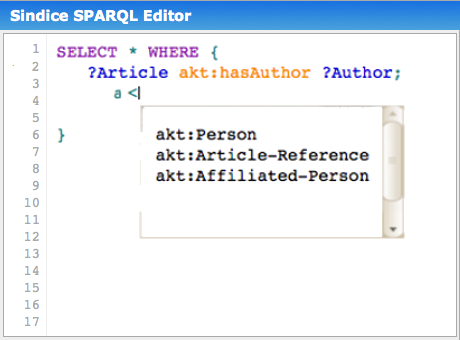
\includegraphics[scale=1]{exploiting/sparqled/figures/sparql/demo1.png}
		}
		\caption{Class}
		\label{fig:rkb-recommendations-types}
	\end{subfigure}
	\begin{subfigure}[t]{.475\textwidth}
		\resizebox{\textwidth}{!}{
			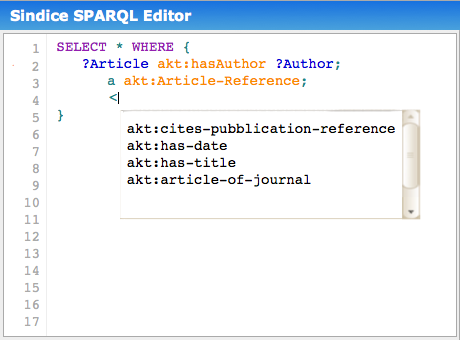
\includegraphics[scale=1]{exploiting/sparqled/figures/sparql/demo2.png}
		}
		\caption{Predicate}
		\label{fig:rkb-recommendations-predicates}
	\end{subfigure}
	\qquad
	\begin{subfigure}[b]{.475\textwidth}
		\resizebox{\textwidth}{!}{
			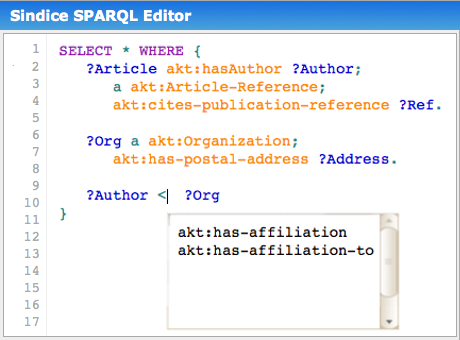
\includegraphics[scale=1]{exploiting/sparqled/figures/sparql/demo3.png}
		}
		\caption{Relationships}
		\label{fig:rkb-recommendations-relations}
	\end{subfigure}
	\begin{subfigure}[b]{.475\textwidth}
		\resizebox{\textwidth}{!}{
			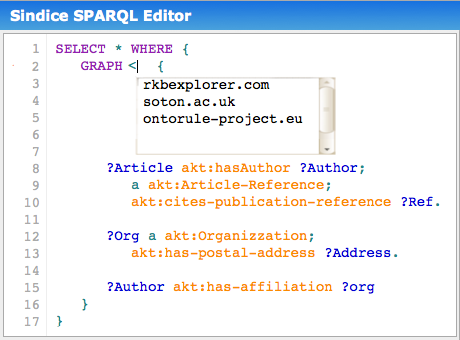
\includegraphics[scale=1]{exploiting/sparqled/figures/sparql/demo4.png}
		}
		\caption{Named Graphs}
    	\label{fig:rkb-recommendations-graph}
	\end{subfigure}
	\caption{Overview of the possible recommendations for the \url{http://www.rkbexplorer.com} dataset depending on the Point of Focus. The Point of Focus is displayed by the green angle bracket $<$.}
  \label{fig:rkb-recommendations}
\end{figure}

\subsection{SPARQL Graph Pattern}

In this section, we introduce the main concepts of SPARQL that are used later in the description of our recommendation engine. SPARQL is the standard query language for RDF data and is based around graph pattern matching. Triple Pattern (TP)~\cite{PrudS08} is the building block in SPARQL:

\begin{definition}[Triple Pattern] A triple pattern is a tuple $t \in (\mathcal{L}^{V^E} \cup Var) \times (\mathcal{L}^A \cup Var) \times (\mathcal{L}^V \cup Var)$ where $\mathcal{L}^{V^E}$ is the set of the entity node labels and $Var$ is an infinite set of variables.
\label{def:triple-pattern}
\end{definition}
The components of a triple pattern $t$ are denoted $subject(t)$, $predicate(t)$ and $object(t)$, respectively.

Triple patterns can be combined into a Basic Graph Pattern (BGP) \cite{PrudS08}. More complex graph patterns can be formed by combining BGPs in various ways~\cite{PrudS08}:\emph{Group Graph Pattern}, \emph{Optional Graph Pattern}, \emph{Alternative Graph Pattern} and \emph{Patterns on Named Graphs}.

A SPARQL query can be translated into an Abstract Syntax Tree (AST). The AST is a tree structure composed of all the logical operators of the query and where leaf nodes are triple patterns to be evaluated. Such an AST is the data structure used by the system to translate the current user needs into possible recommendations. In our implementation, the AST can contain an incomplete TP and a special symbol `$<$' to indicate the POF.

\subsection{From Data Graph to Data Graph Summary}

In order to suggest the possible structural elements to the user with respect to the current state of his query, we need to translate the AST of the query into another AST compatible with the data graph summary. This new AST is then evaluated on the data graph summary and the possible structural elements are retrieved and presented to the user. The AST translation is performed in three steps: 
\begin{inparaenum}
\item transformation of the POF symbol `$<$' into a variable to project as the query solution; 
\item removal of content elements from the AST; and
\item mapping of triple patterns into \emph{summary patterns}.
\end{inparaenum}
Figure~\ref{fig:entity-gs-sparql} depicts a translation of a data graph query (Figure~\ref{fig:entity-sparql}) to a data graph summary query (Figure~\ref{fig:gs-sparql}).

\begin{figure}

\newsavebox{\sparql}
\begin{lrbox}{\sparql}
\begin{minipage}{0.3\textwidth}
\centering
%% Because of syntax error in the query, and also becaus empty prefixes are not supported
\expandafter\def\csname PY@tok@err\endcsname{}
\begin{minted}[linenos,frame=lines,framesep=4mm]{sparql}
SELECT * WHERE {
 ?a a p:Article ;
    :title ?t .



 ?i a :Institute ;
    :employs ?p .



 ?p :name "Renaud" ;



    <


}
\end{minted}
\label{lst:sparql}
\end{minipage}
\end{lrbox}


\newsavebox{\sparqlSum}
\begin{lrbox}{\sparqlSum}
\begin{minipage}{0.4\textwidth}
\centering
\begin{minted}[linenos,frame=lines,framesep=4mm,]{sparql}
SELECT ?POF WHERE {
 ?a :label :Article .
 ?x :label :title ;
    :source ?a ;
    :target ?t .

 ?i :label :Institute .
 ?y :label :employs ;
    :source ?i ;
    :target ?p .

 ?z1 :label :name ;
     :source ?p ;
     :target ?_z1 .

 ?z2 :label ?POF ;
     :source ?p ;
     :target ?_z2 .
}
\end{minted}
\label{lst:gs-sparql}
\end{minipage}
\end{lrbox}

\begin{tabular}{crccr}
\phantom{a}
 &
 \begin{subfigure}[t]{.275\textwidth}
		\usebox{\sparql}
 		\caption{SPARQL query over the data graph. The Point of Focus is depicted by the angle bracket $<$.}
 		\label{fig:entity-sparql}
\end{subfigure} 
 & \phantom{a} & \phantom{a} &
 \begin{subfigure}[t]{.55\textwidth}
	 \usebox{\sparqlSum}
 	\caption{SPARQL query over the data graph summary. The Point Of Focus defines the solution set, i.e., the variable $?POF$ in the SELECT clause.}
 	\label{fig:gs-sparql}
 \end{subfigure}
 \\
\end{tabular}
\caption{Mapping from a data graph query to a data graph summary query.}
\label{fig:entity-gs-sparql}
\end{figure}

\subsubsection{Summary Pattern}

Similar to Triple Patterns in SPARQL, Summary Patterns (SPs) are the building blocks to construct a data graph summary query.

\begin{definition}[Summary Pattern] 
A \emph{Summary Pattern} is a tuple $t \in  (\mathcal{L}^C \cup Var) \times (\mathcal{L}^A \cup Var) \times (\mathcal{L}^C \cup Var)$.
\label{def:summary-triple-pattern}
\end{definition}

With respect to our RDF data model of the data graph summary, such a summary pattern is translated into a SPARQL BGP. For example, given the SP \mbox{$<Institute, employs, ?p>$}, the corresponding SPARQL BGP is equal to the BGP in Figure~\ref{fig:gs-sparql} from the line 7 to line 10.

\subsubsection{Projection of POF}

The first step consists of defining the variable to project as the query solution. In the TP containing the POF, we transform the POF symbol into a variable $?POF$ and complete that TP with a wildcard variable if needed (we denote by wildcard variable a variable that is unique in the query). For example in Figures~\ref{fig:entity-sparql} and~\ref{fig:gs-sparql} at line 16, the POF symbol `$<$' is translated into the variable $?POF$, and the wildcard variable $?\_z2$ is added to complete the triple pattern.
The initial \emph{Query Form}~\cite{PrudS08} of the AST is replaced by a projection of the POF variable using the \emph{SELECT} form.

\subsubsection{Removal of content elements}

The second step consists in removing all content elements from the AST. A content element is an element that describes a specific aspect of an entity, thus it does not inform about its structure. We replace with a wildcard variable Literals and URIs that appear in a TP at a subject or object position, except if the TP is a \emph{Class Triple Pattern} (CTP). In that case, only the element at the subject position is replaced by a wildcard variable. For instance, the literal ``Renaud'' in Figure~\ref{fig:entity-sparql} is replaced by the variable $?\_z1$ in Figure~\ref{fig:gs-sparql}.

\begin{definition}[Class Triple Pattern] 
A \emph{Class Triple Pattern} is a triple pattern $t$ such as $predicate(t) \in \mathcal{L}^{A_c}$.
\label{def:class-triple-pattern}
\end{definition}

\subsubsection{Mapping}

The third step consists in mapping all triple patterns into summary patterns, according to the following two rules. If the triple pattern $<var_s, p, o>$ is a CTP, then it is replaced with a new triple pattern \mbox{$<var_s, label, o>$}. Otherwise, the triple pattern \mbox{$<var_s, p, var_o>$} is replaced with the following BGP:

\begin{enumerate}
    \item A new wildcard variable $var_x$, representing an edge node $x$, is created;
    \item A triple pattern $<var_x, source, var_s>$ is created to set the source of the edge;
    \item A triple pattern $<var_x, target, var_o>$ is created to set the target of the edge;
    \item A triple pattern $<var_x, label, p>$ is created to set the label of the edge.
\end{enumerate}

In the case where the triple pattern $<var_s, p, var_o>$ belongs to a \emph{Graph Graph Pattern}~\cite{PrudS08}, i.e., a group graph pattern associated to a named graph URI $g$ with the \emph{GRAPH} operator, then a triple pattern $<var_x, origin, g>$ is added to the previously defined BGP to set the named graph of the edge. However, if the named graph is the POF variable, the triple pattern $<var_x, origin, var_{POF}>$ is created instead in order to restrict each edge to be from the same dataset and to bind the dataset label to the POF variable.

Applying these mapping rules on the query of Figure~\ref{fig:entity-sparql}, the first TP \mbox{$<var_a, a, Article>$}, being a CTP, is translated into the SP \mbox{$<var_a, :label, Article>$}. The second TP \mbox{$<var_a, :title, var_t>$} is translated into the BGP from line 3 to line 5 of the query displayed in Figure~\ref{fig:gs-sparql}.

\subsection{Recommendation Scope}

In certain cases during the formulation of a query, the query may contain multiple BGPs, among which one does not return any result. The system will therefore no longer produce recommendations, as the evaluation of the data graph summary query will also not produce any results. However, this can be interpreted incorrectly by the user since he might believe that the dataset does not contain any other information. In order to minimise this issue, we introduce the notion of \emph{recommendation scope}.

The \emph{recommendation scope} helps to reduce the extent of the area that is relevant for the recommendation. Instead of taking into account the full SPARQL query, the recommendation engine will take only a relevant subset. The recommendation scope is defined recursively by including all the triple patterns with a path to the POF variable. A \emph{breadth-first search} algorithm on the query, starting on the POF node, is performed in order to find all the graph components that are connected to the POF. All the graph components that are not connected to the POF are removed. This prevents non-relevant (to the POF) triple patterns from limiting the recommendations. For example, in Figure~\ref{fig:entity-sparql}, the recommendation scope does not contain the first BGP since it is not connected to the POF variable, whether directly or indirectly. Another possible solution for this issue is to provide to the user an estimation of the cardinality of TPs or BGPs that can lead to an empty result set. This is possible given the cardinality information provided by the data graph summary. We are currently planning to investigate this solution for future works.


\subsection{Entity Authority}
\todo{move this to the applications part}

When working with the Web of Data, it is legitimate to wonder about the quality of the data. The quality not according to whether the data follows modelling standards or not, but rather to the information itself. Indeed, in an environment where data can be edited by anybody, it can happen that some statements about an entity, or relationships between two entities, can be erroneous. Therefore, there is a need to define the \emph{authority} of an entity in order to judge how much confidence one can put in the information about the entity that a dataset provides.\todo{Define the dataset set}

\begin{definition}[Entity Authority]
Let $v \in V$ an entity and $a_v : V \mapsto \mathcal{L}^D$ a function which assigns a dataset label to an entity, called the entity \emph{authority}. Statements about an entity are then said \emph{authoritative} if the dataset label given by $a_v$ and the label of the dataset where the statements are found are the same.
\end{definition}

For example, the authority of an entity is \emph{D1}, but a statement about that entity is found in a dataset labelled \emph{D2}; the validity of that statement should then be checked.
